\documentclass[a4paper,12pt]{article}
\usepackage{amsmath}
\usepackage{graphicx}
\usepackage{siunitx}
\usepackage{float}

\title{Freezing Point Depression of Salt Solutions}
\author{Group 304: Simone Keldenich, Lukas Othmann, Kilian Mandon}
\date{16.09.2024}

\begin{document}

\maketitle

\section{Introduction}
Freezing point depression is a colligative property of solutions, meaning it depends on the number of solute particles present in the solvent rather than the identity of the solute. When a non-volatile solute is dissolved in a solvent, the freezing point of the solution is lower than that of the pure solvent. This occurs because the presence of solute particles disrupts the formation of the solid crystalline structure of the solvent, requiring a lower temperature to reach the solid phase.

During the freezing process of a pure solvent, supercooling can occur, where the liquid is cooled below its freezing point without forming a solid. Once nucleation begins and freezing occurs, the temperature rises to the equilibrium freezing point due to the release of latent heat. This temperature remains constant during the phase transition as the system reaches a dynamic equilibrium where the rates of freezing and melting are equal.

The depression in freezing point can be quantified using the formula:

\begin{equation}
\Delta T_f = K_f \cdot m,
\end{equation}

where $\Delta T_f$ is the freezing point depression, $K_f$ is the cryoscopic constant of the solvent, and $m$ is the molality of the solution. The cryoscopic constant is a property of the solvent and depends on its chemical nature and structure.

In this experiment, we aim to determine the molar mass of a salt by measuring the freezing point depression of water as a solvent. The relationship between the freezing point depression and the molar mass of the solute is given by:

\begin{equation}
M_2 = \frac{\theta \cdot \frac{m_{\text{solute}}}{m_{\text{solvent}}}}{\Delta T} \times 2,
\end{equation}

where $M_2$ is the molar mass of the solute, $\theta$ is the cryoscopic constant of the solvent, $\frac{m_{\text{solute}}}{m_{\text{solvent}}}$ is the mass ratio of solute to solvent, and $\Delta T$ is the observed freezing point depression. The factor of 2 accounts for the binary nature of the salt, assuming complete dissociation.

\section{Methods}
To measure the freezing point depression of water upon the addition of salt, we prepared three different solutions of varying salt concentrations. The salt used in this experiment has the general formula MX, where M is an alkali metal and X is a halogen. The masses of the salt were weighed precisely as follows: 1.000 g, 2.000 g, and 3.000 g. Each sample was dissolved in 100 mL of deionized water using a volumetric pipette.

The mass of the solvent was calculated using the density of water at room temperature, which was measured to be 21.4°C. The density was determined using the formula:

\begin{equation}
\rho = -0.00022897 \cdot T + 1.00277688,
\end{equation}

where $T$ is the temperature in degrees Celsius, and $\rho$ is the resulting density in g/mL.

To create a cooling bath, a 2L beaker was filled halfway with ice, and water was added up to approximately 1.8 L. A larger magnetic stir bar was placed in the beaker to ensure proper mixing. To lower the temperature of the bath to between -3°C and -4°C, thawing salt was added.

First, the freezing point of the pure solvent (water) was determined. Approximately 30-40 mL of deionized water was placed in a sample container equipped with a smaller magnetic stir bar. The container was sealed with a rubber stopper, through which a thermocouple was inserted. The thermocouple was connected to a digital thermometer to monitor the temperature. The sample container was placed in the cooling bath, and the magnetic stirrer was activated. The temperature was recorded as it decreased. When nucleation occurred, indicated by a sudden rise in temperature, the stirrer was turned off, and the temperature was monitored until it stabilized, indicating the equilibrium freezing point. This measurement was repeated three times with freshly filled water each time to obtain an average value.

Following the pure solvent measurements, the freezing points of the three salt solutions were measured. The solutions were prepared by dissolving the weighed salt masses in 100 mL of deionized water. Each solution was placed in the sample container and cooled in the same manner as the pure solvent. The temperature of each solution was recorded at the equilibrium point, and measurements were repeated three times for each concentration to ensure accuracy.

\section{Results}
In this experiment, we measured the freezing point depression of water upon the addition of different masses of a salt. From these measurements, we calculated the molar mass of the salt using the cryoscopic constant. All calculations included Gaussian error propagation to determine the uncertainties in the results.

\subsection{Measured and Calculated Values}
The room temperature during the experiment was measured as:
\begin{equation}
T_{\text{room}} = 21.40 \pm 0.10 \, ^\circ\text{C}.
\end{equation}

Using the temperature, the density of the solvent (water) was calculated using the formula:
\begin{equation}
\rho(T) = (-0.00022897 \, \text{g/mL} \cdot ^\circ\text{C}^{-1}) \cdot T + 1.00277688 \, \text{g/mL}.
\end{equation}

Substituting the measured temperature, the density of the solvent was found to be:
\begin{equation}
\rho_{\text{solvent}} = 0.997877 \pm 0.000093 \, \text{g/mL}.
\end{equation}

The mass of the solvent was then calculated using the formula:
\begin{equation}
m_{\text{solvent}} = V_{\text{solvent}} \cdot \rho_{\text{solvent}},
\end{equation}
where $V_{\text{solvent}}$ is the volume of the solvent. Given that the volume was $100.0$ mL, the mass of the solvent was:
\begin{equation}
m_{\text{solvent}} = 99.79 \pm 0.01 \, \text{g}.
\end{equation}

\subsection{Freezing Point Measurements}
The average freezing point of the pure solvent (water) was measured as:
\begin{equation}
T_{\text{pure}} = 0.59 \pm 0.01 \, ^\circ\text{C}.
\end{equation}

For each salt solution, the freezing point and the freezing point depression were measured and calculated as follows:

\begin{itemize}
    \item \textbf{Salt Mass: 1.00 g}
    \begin{align*}
    T_{\text{solution, 1g}} &= 0.09 \pm 0.01 \, ^\circ\text{C}, \\
    \Delta T_1 &= T_{\text{pure}} - T_{\text{solution, 1g}} = 0.49 \pm 0.02 \, ^\circ\text{C}.
    \end{align*}

    \item \textbf{Salt Mass: 2.00 g}
    \begin{align*}
    T_{\text{solution, 2g}} &= -0.40 \pm 0.01 \, ^\circ\text{C}, \\
    \Delta T_2 &= T_{\text{pure}} - T_{\text{solution, 2g}} = 0.99 \pm 0.02 \, ^\circ\text{C}.
    \end{align*}

    \item \textbf{Salt Mass: 3.00 g}
    \begin{align*}
    T_{\text{solution, 3g}} &= -0.84 \pm 0.03 \, ^\circ\text{C}, \\
    \Delta T_3 &= T_{\text{pure}} - T_{\text{solution, 3g}} = 1.43 \pm 0.03 \, ^\circ\text{C}.
    \end{align*}
\end{itemize}

\subsection{Molar Mass Calculation}
The molar mass of the salt was calculated using the equation:
\begin{equation}
M_2 = \frac{\theta \cdot \frac{m_{\text{solute}}}{m_{\text{solvent}}}}{\Delta T} \times 2,
\end{equation}
where $\theta$ is the cryoscopic constant of water, $1858 \, \text{g} \cdot \text{K/mol}$, $\frac{m_{\text{solute}}}{m_{\text{solvent}}}$ is the mass ratio of the solute to the solvent, and $\Delta T$ is the freezing point depression. 

The calculated molar masses and their errors for each solution were:

\begin{itemize}
    \item \textbf{Salt Mass: 1.00 g}
    \begin{equation*}
    M_2 = 75.48 \pm 2.61 \, \text{g/mol}.
    \end{equation*}

    \item \textbf{Salt Mass: 2.00 g}
    \begin{equation*}
    M_2 = 75.48 \pm 1.23 \, \text{g/mol}.
    \end{equation*}

    \item \textbf{Salt Mass: 3.00 g}
    \begin{equation*}
    M_2 = 78.31 \pm 1.70 \, \text{g/mol}.
    \end{equation*}
\end{itemize}

The mean molar mass, calculated from all measurements, was:
\begin{equation}
M_{\text{mean}} = 76.43 \pm 1.12 \, \text{g/mol},
\end{equation}
with a standard deviation of $1.63 \, \text{g/mol}$.

\subsection{Graphical Representation}
Figure \ref{fig:molar_mass_plot} shows the molar masses plotted against the mass of the salt used in each solution, including the error bars for each measurement.

\begin{figure}[H]
    \centering
    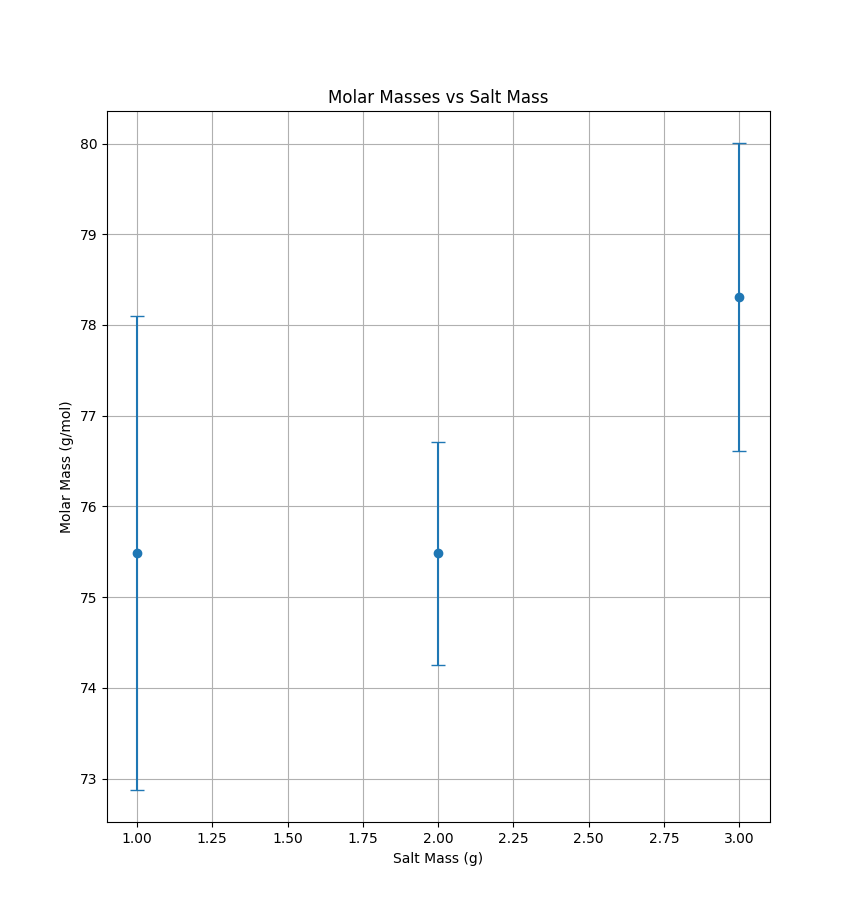
\includegraphics[width=\textwidth]{images/molar_mass_by_salt_mass.png}
    \caption{Molar mass of the salt as a function of the mass of salt used in the solution. Error bars indicate the uncertainties in the calculated molar masses.}
    \label{fig:molar_mass_plot}
\end{figure}

This plot demonstrates the consistency of the molar mass determination across different concentrations of the salt, with the molar mass remaining relatively constant despite variations in salt mass.

\section{Discussion}
The goal of this experiment was to determine the molar mass of a salt using the freezing point depression method. Our results yielded a mean molar mass of:
\begin{equation}
M_{\text{mean}} = 76.43 \pm 1.12 \, \text{g/mol},
\end{equation}
with a standard deviation of $1.63 \, \text{g/mol}$.

\subsection{Error Analysis}
The propagated error in our calculated mean molar mass was $1.12 \, \text{g/mol}$, while the standard deviation of the molar mass values was $1.63 \, \text{g/mol}$. The standard deviation being larger than the propagated error indicates that there was some variability in the measurements beyond what was expected from the error propagation alone. This could be due to experimental factors such as:
\begin{itemize}
    \item Slight variations in the actual temperature of the cooling bath during measurements,
    \item Minor inaccuracies in weighing the salt or solvent,
    \item Potential supercooling effects leading to slight differences in observed freezing points.
\end{itemize}
Despite these factors, the standard deviation and the propagated error are relatively close, suggesting that the experimental setup and the error analysis were reasonably reliable.

\subsection{Comparison with Potassium Chloride}
The molar mass we obtained, $76.43 \, \text{g/mol}$, is close to that of potassium chloride (KCl), which has a molar mass of $74.56 \, \text{g/mol}$. The small difference between the measured molar mass and that of KCl could be attributed to experimental uncertainties or minor impurities in the salt used. Considering the cryoscopic method's inherent limitations, this result suggests that the salt used in the experiment was likely KCl or a compound with a very similar molar mass.

Given that potassium chloride is a common salt with a simple binary ionic structure (dissociating into K\textsuperscript{+} and Cl\textsuperscript{-} ions), it is plausible that the observed colligative properties and the derived molar mass correspond to this salt. Therefore, the experiment was successful in not only determining the molar mass of the unknown salt but also in identifying it as a compound very similar to KCl.

\subsection{Conclusion}
The experiment effectively demonstrated the freezing point depression method for determining the molar mass of an unknown salt. While there was some variability in the measurements, the final molar mass value was reasonably consistent with the known molar mass of potassium chloride, suggesting that the salt used was KCl or a similar compound. This outcome shows the utility of colligative properties in practical chemical analysis and reinforces the importance of careful measurement and error analysis in experimental chemistry.

\end{document}